\subsection*{Problema 29}
\textbf{Enunciado:} Calcular la integral:
\begin{align*}
\int \dfrac{2x^3 + 3x^2 + x - 1}{(x + 1)(x^2 + 2x + 2)^2} \, dx
\end{align*}

\textbf{Solución:} 
El integrando es una función racional propia. 
Utilizamos el método de fracciones parciales:
\begin{align*}
\dfrac{2x^3 + 3x^2 + x - 1}{(x + 1)(x^2 + 2x + 2)^2} = \dfrac{A}{x + 1} \\
+ \dfrac{Bx + C}{x^2 + 2x + 2} + \dfrac{Dx + E}{(x^2 + 2x + 2)^2}
\end{align*}

Multiplicando por el denominador común e igualando numeradores, evaluando en $x = -1$ obtenemos $A = 1$. 
Para los demás coeficientes, expandimos y agrupamos términos semejantes, resultando en:
$B = 1$, $C = 0$, $D = 1$ y $E = 1$. 
Sustituyendo los valores:
\begin{align*}
\int \left( \dfrac{1}{x + 1} + \dfrac{x}{x^2 + 2x + 2} \right. \\
\left. + \dfrac{x + 1}{(x^2 + 2x + 2)^2} \right) dx
\end{align*}

Integramos cada término por separado. 
Para el segundo término, completamos el diferencial del denominador:
\begin{align*}
\int \dfrac{x}{x^2 + 2x + 2} \, dx = \dfrac{1}{2}\ln(x^2 + 2x + 2) \\
- \arctan(x + 1)
\end{align*}

Para el tercer término, usamos la sustitución trigonométrica sugerida $x + 1 = \tan(\theta)$:
\begin{align*}
\int \dfrac{x + 1}{((x + 1)^2 + 1)^2} \, dx = -\dfrac{1}{2(x^2 + 2x + 2)}
\end{align*}

Combinando todos los resultados y añadiendo la constante de integración $C$, obtenemos la solución general:
\begin{align*}
I = \ln|x + 1| + \dfrac{1}{2}\ln(x^2 + 2x + 2) \\
- \arctan(x + 1) - \dfrac{1}{2(x^2 + 2x + 2)} + C
\end{align*}

\begin{figure}[H]
	\centering
	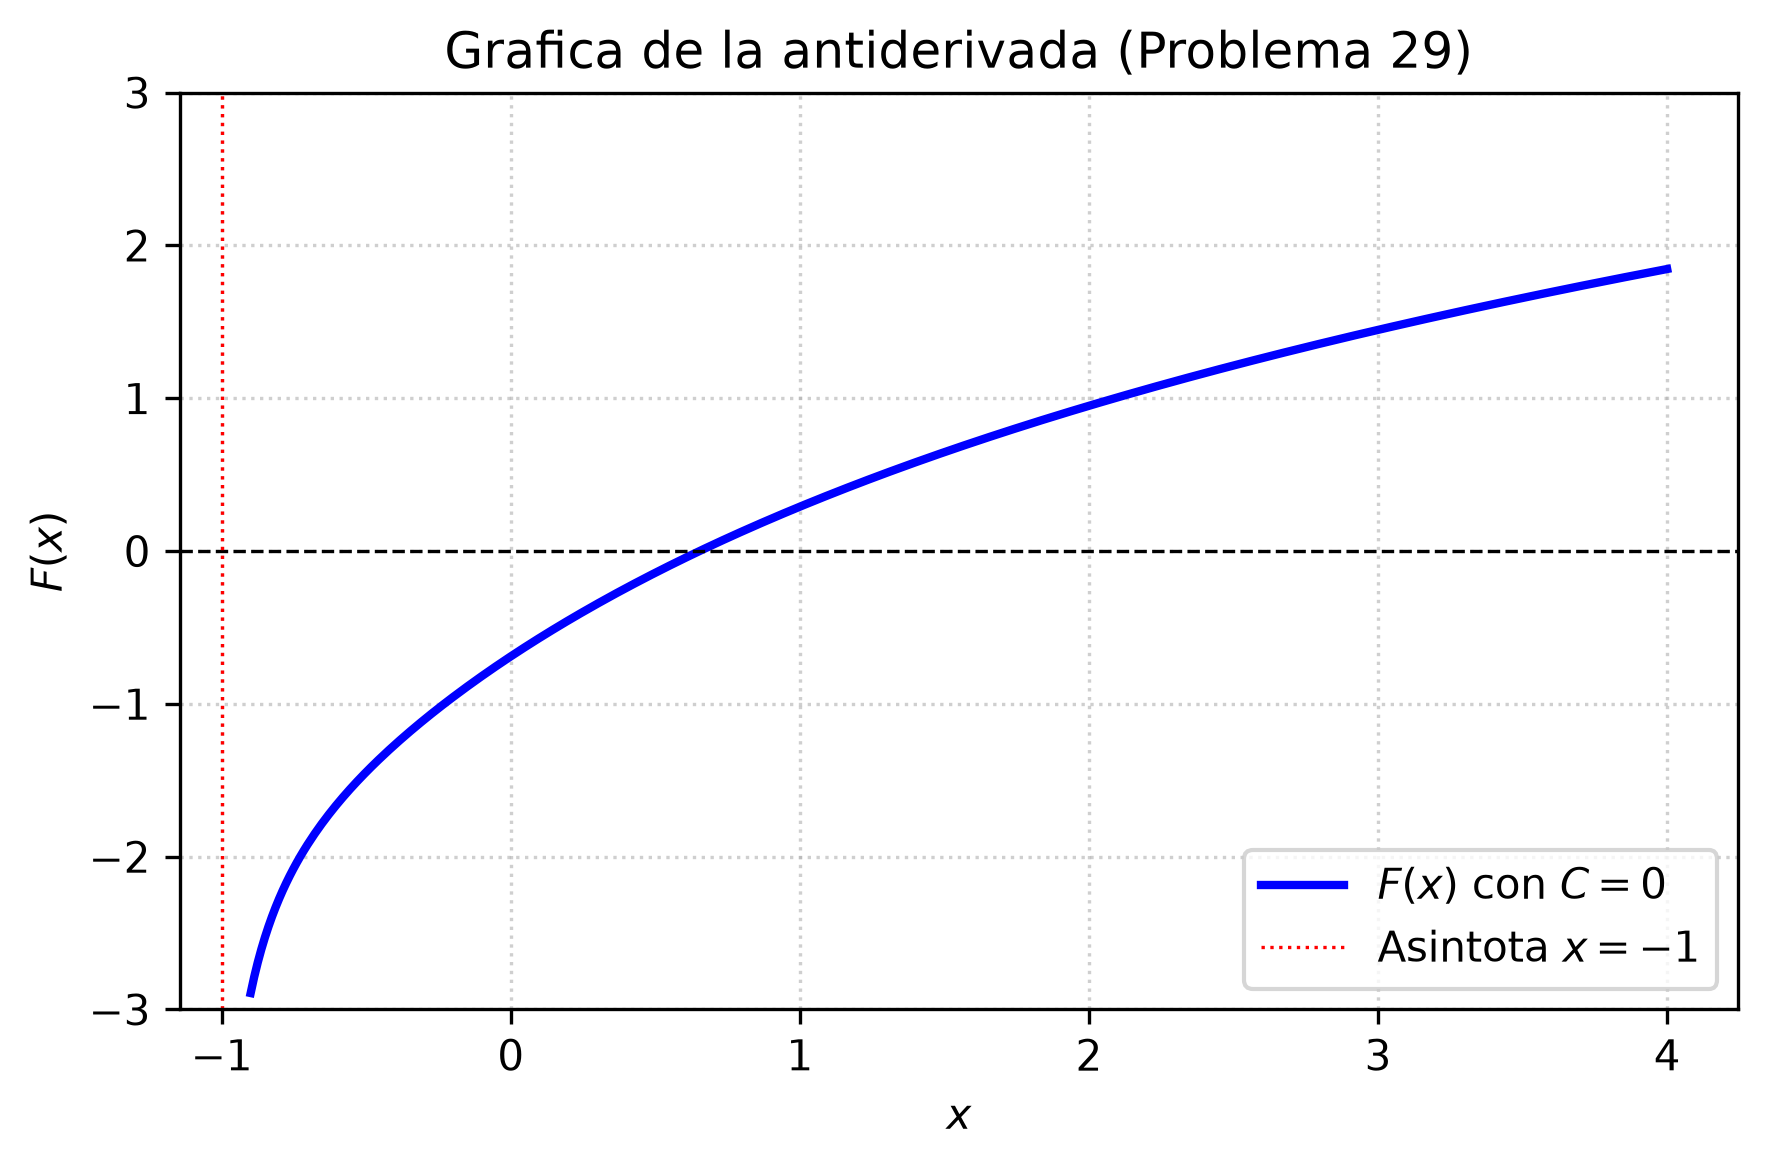
\includegraphics[width=\columnwidth]{semana_03/graficas/SEM03_P29_grafica.png}
	\caption{Representación gráfica de $f(x)$ y su antiderivada $F(x)$ evaluada para la constante de integración $C = 0$ (Problema 29).}
	\label{fig:problema29}
\end{figure}
